\chapter{Weryfikacja i walidacja}
\label{ch:06}
\section{Sposób testowania w ramach pracy}
Podczas rozwoju systemu na bieżąco były wykonywane testy integracyjne mające na celu walidację poprawności działania zaimplementowanych komponentów. 

Dodatkowo przeprowadzony został test wydajnościowy, w którym zmierzona została ilość użytej pamięci RAM przez uruchomioną aplikację, do której trafiały 4 różne zapytania co 20ms. Wyniki zaprezentowane na Rys. \ref{fig:performance} pokazują, że aplikacja najwięcej zasobów zużyła podczas uruchomienia, a w ciągu normalnego działania zużywane są niewielkie ilości.
\begin{figure}[h]
\centering
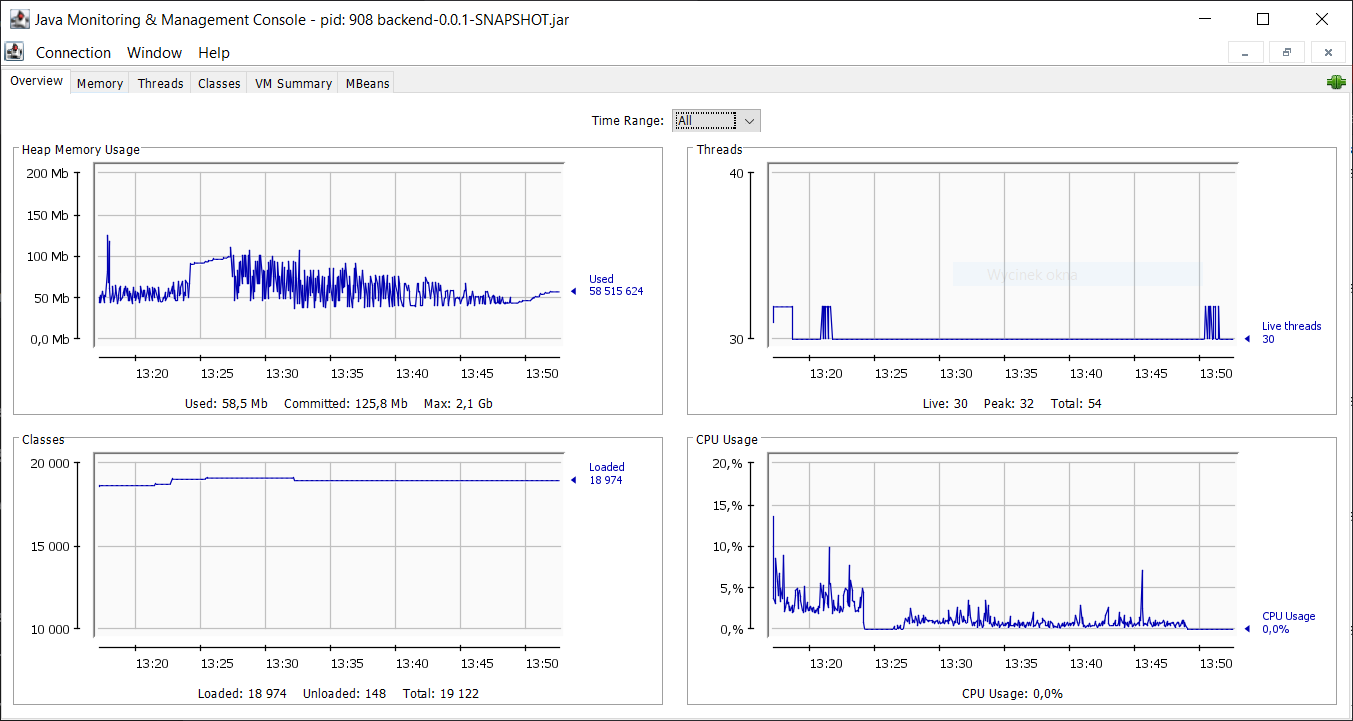
\includegraphics[width=0.95\textwidth]{./graf/performance.PNG}
\caption{Wyniki testu wydajnościowego}
\label{fig:performance}
\end{figure}

\section{Organizacja eksperymentów}
Aby przeprowadzić testy użyte zostało narzędzie Postman, które umożliwia tworzenie oraz wysyłanie żądań HTTP do serwera z ustawionymi danymi, nagłówkami oraz parametrami i pozwala odczytać otrzymane wyniki. Narzędzie to pozwoliło na bieżące testy API bez konieczności implementacji interfejsu użytkownika. Platforma została także użyta w teście wydajnościowym, aby symulować ruch w sieci.

Pomiary wydajnościowe zostały wykonane przy użyciu konsoli monitorowania i zarządzania w Javie, która umożliwia monitorowanie aplikacji oraz zbieranie danych diagnostycznych. 

Dodatkowo podczas implementacji interfejsu użytkownika, wykorzystane zostało narzędzie inspektora dostępne w przeglądarce internetowej.

\section{Przypadki testowe, zakres testowania}
W aplikacji serwera przetestowane zostały wszystkie punkty końcowe pod względem poprawności przyjmowanych danych (niepoprawna długość, niedozwolone znaki, puste lub wypełnione białymi znakami łańcuchy znaków itp.), dodatkowo sprawdzone zostało czy zapytania, które odnoszą się do nieistniejących danych są poprawnie odrzucane (nieistniejące sesje, użytkownicy itp.). Punkty końcowe aplikacji serwera zostały przetestowane także pod względem bezpieczeństwa - nieważny token bezpieczeństwa lub jego całkowity brak czy próby dostępu do niedozwolonych dla danej kategorii użytkowników funkcjonalności takiej jak sterowanie odtwarzaczem muzyki przez gościa sesji. Przetestowana została także poprawność działania zasad sesji, które blokują użytkownikom dodawanie utworów ponad ustawiony limit czy dołączanie do sesji, która jest już pełna.

\section{Wykryte i usunięte błędy}
Podczas implementacji systemu wykryto oraz usunięto stosunkowo dużo błędów, najczęściej występowały w kodzie aplikacji serwera. Przykładem może być błąd, który powodował odrzucanie wszystkich zapytań pochodzących z aplikacji klienta przez serwer. Błąd nie występował podczas korzystania z narzędzi do testowania API, lecz pojawił się w momencie implementacji interfejsu użytkownika. Przyczyną okazał się źle skonfigurowany moduł odpowiedzialny za kontrolę dostępu. Przeglądarka zanim wyśle do serwera właściwe żądanie wysyła zapytanie typu OPTIONS, który jest częścią mechanizmu bezpieczeństwa przeglądarki. Aplikacja serwera odrzucała wszystkie zapytania bez nagłówka autoryzacji w tym wszystkie zapytanie typu OPTIONS, bez których komunikacja jest niemożliwa. Kilka błędów, które się pojawiły były spowodowane literówkami bądź użyciem złej funkcji o podobnej nazwie, przez co program się kompilował, lecz nie działał poprawnie.

W interfejsie użytkownika wykryto i usunięto wiele błędów związanych ze stylem takie jak źle ułożone elementy czy niepoprawnie wyświetlające się moduły. Usunięte zostały także błędy związane z komunikacją z aplikacją serwera, które uniemożliwiały poprawną autoryzację czy korzystanie z niektórych funkcjonalności systemu.

